%!TEX root = ../thesis.tex

\chapter{闪电氮氧化物产率的估算} \label{chapter:PE}

\section{清洁地区(北极)}

\subsection{闪电的分布}
\subsection{反演闪电氮氧化物的步骤}
\subsection{闪电氮氧化物的聚类}
\subsection{闪电氮氧化物浓度与其他氮氧化物源的对比}
\subsection{闪电氮氧化物的寿命及产率}
\subsection{不确定性分析}


\section{污染地区(中国及美国大陆)}

\subsection{模式设置}

使用的WRF-Chem版本为3.5.1,水平网格大小为12 km $\times$ 12 km (图\ref{us_domain}(a)),垂直层数为29层,时间步长为72 s。
气象条件的初始场和边界场为时间分辨率3小时的北美区域再分析(NARR)数据集,每3小时应用一次边界条件和四维数据分析(FDDA)逼近,
其中温度、水汽和水平风以0.0003 s$^{-1}$ 的系数逼近\citep{Laughner.2017}。
微物理过程采用Lin方案\citep{Lin.1983},积云参数化为Grell 3D方案\citep{Grell.1993a,Grell.2002a},长波辐射采用RRTM方案\citep{Iacono.2008},短波辐射采用Goddard方案,陆面过程使用Noah陆面模式\citep{Koren.1999},边界层采用YSU方案\citep{Hong.2006}。
闪电参数化采用基于对流参数化的中性浮力水平\citep{Pickering.1992},云闪与地闪的比例基于\citet{Boccippio.2001}.

采用臭氧和相关化学示踪剂模型第4版(MOZART-4;\citet{Emmons.2010})的输出场作为化学的初始场和边界场。
人为排放由2011年美国国家排放清单(NEI)驱动,并根据环境保护署年度总排放量,按模拟的年份进行调整\citep{EPA.2015}。
生物排放使用MEGAN源,化学机制是区域大气化学机制第2版(RACM2;\citet{Goliff.2013}),并由\citet{Browne.2014}和\citet{Schwantes.2015}进行了更新。
此外,LNO$_x$参数化采用每次闪电产生200 mol NO,调整因子为1,以下简称“1$\times$200 mol NO per flash”)。
基于\citet{Ott.2010}的双峰型闪电NO(LNO)廓线\citep{Laughner.2017}被用作 WRF-Chem中LNO的垂直分布,而LNO和LNO$_2$廓线是指有和没有闪电的模拟之间垂直廓线的差异。


\begin{figure}[h]
\centering
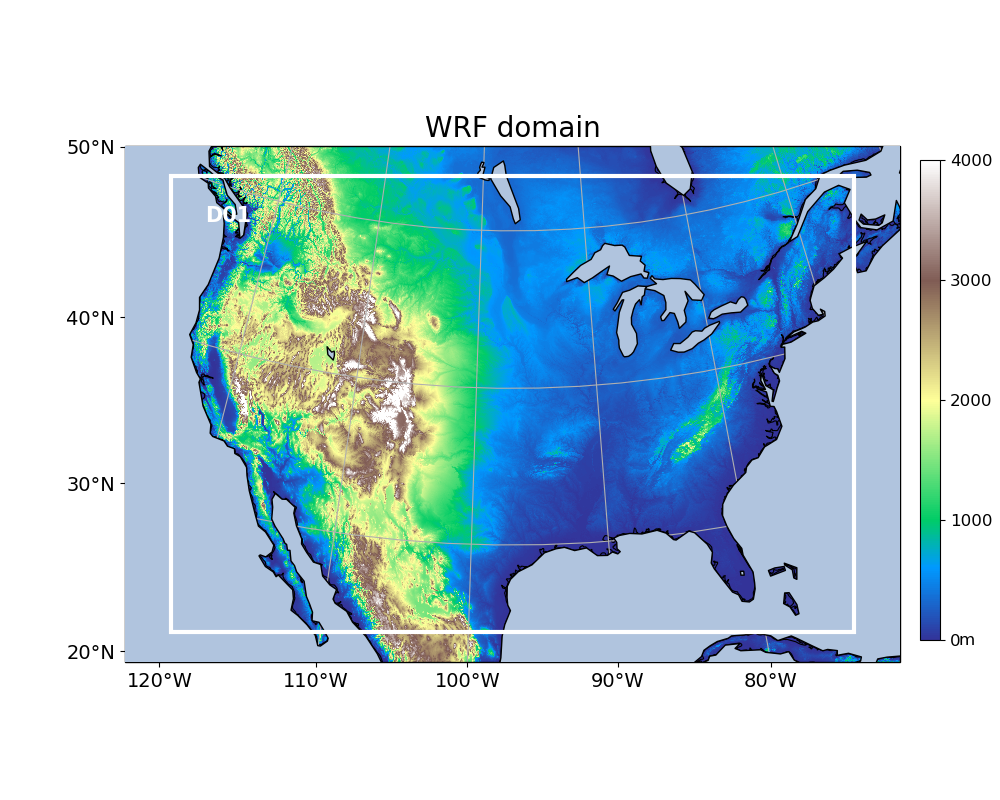
\includegraphics[width=12cm]{./figures/us_domain.png}
\caption{WRF-Chem 模拟区域和地形高度 (m),网格数为 350 $\times$ 290,水平分辨率为 12 km \\
Figure \ref{fig:us_domain}. Domain and terrain height (m) of the WRF-Chem simulation with 350 x 290 grid cells and a horizontal resolution of 12 km.}
\label{fig:us_domain}
\end{figure}


\subsection{反演闪电氮氧化物的步骤}

首先我们使用恒定值网格化法,将公式(\ref{eq:AMF_LNO2})所得的LNO$_x$垂直柱密度(V$_{\textrm{NO$_x$}}$)分配至0.05$^{\circ}$ $\times$ 0.05$^{\circ}$网格\citep{Kuhlmann.2014}。
接着在 1$^{\circ}$ $\times$ 1$^{\circ}$的网格中进行分析,要求每个网格至少有50个有效的0.05$^{\circ}$ $\times$ 0.05$^{\circ}$网格数据,从而最小化噪点数据。
具体LNO$_x$的主要计算步骤如下。

云辐射分数(CRF,CRF $\geq$ 70\%,CRF $\geq$ 90\%,CRF = 100\%)和 云压(CP,CP $\leq$ 650 hPa)是OMI像素是否包含深对流云的判断标准\citep{Ziemke.2009,Choi.2014,Pickering.2016}。
不同CRF对LNO$_x$产品的影响将在\ref{subsec:criteria}节探讨。
此外,我们将另一个云分数 (CF) 标准应用于 WRF-Chem 的模拟结果,以确保对流被成功模拟。
具体而言,CF是由 Xu-Randall 方法计算的 350--400 hPa 之间的最大云分数\citep{Xu.1996,Strode.2017}。
选择350--400 hPa的大气层,可避免模拟高云中的偏差。
我们选择\citet{Strode.2017}建议的 CF $\geq$ 40\%来判断模拟所处的网格是多云或晴空。

除了云特性之外,OMI能探测到新生LNO$_x$的另一条件为一段时间内有足够的闪电或闪击。
其中,时间窗口 (t$_{window}$) 是 OMI 过境之前的时间段。
\citet{Lapierre.2020}利用1$^{\circ}$ $\times$ 1$^{\circ}$网格的对角线长度和OMI过境时美国大陆上空500--100 hPa的平均风速计算得到t$_{window}$为2.4 h。
同时,\citet{Lapierre.2020}定义在t$_{window}$时间段内,至少发生2400次闪电或8160次闪击的网格才能提供足够的LNO$_x$给OMI探测。
\citet{Bucsela.2019}的研究表明,低频率的闪电具有更高的LNO$_x$产率(PE),而该段数据在\citet{Lapierre.2020}研究中被剔除。
通过比较使用每个网格至少2400次闪电和至少1次闪电的标准所得结果,我们也得到相同的结论(图\ref{fig:flash_threshold})。
由于我们的研究重点是开发一种新的空气质量转换因子(AMF),并将计算结果与使用类似闪电阈值的其他产品进行比较\citep{Pickering.2016,Lapierre.2020},
因此我们接下来使用相同的至少2400次闪电标准来进行结果分析。


\begin{figure}[h]
    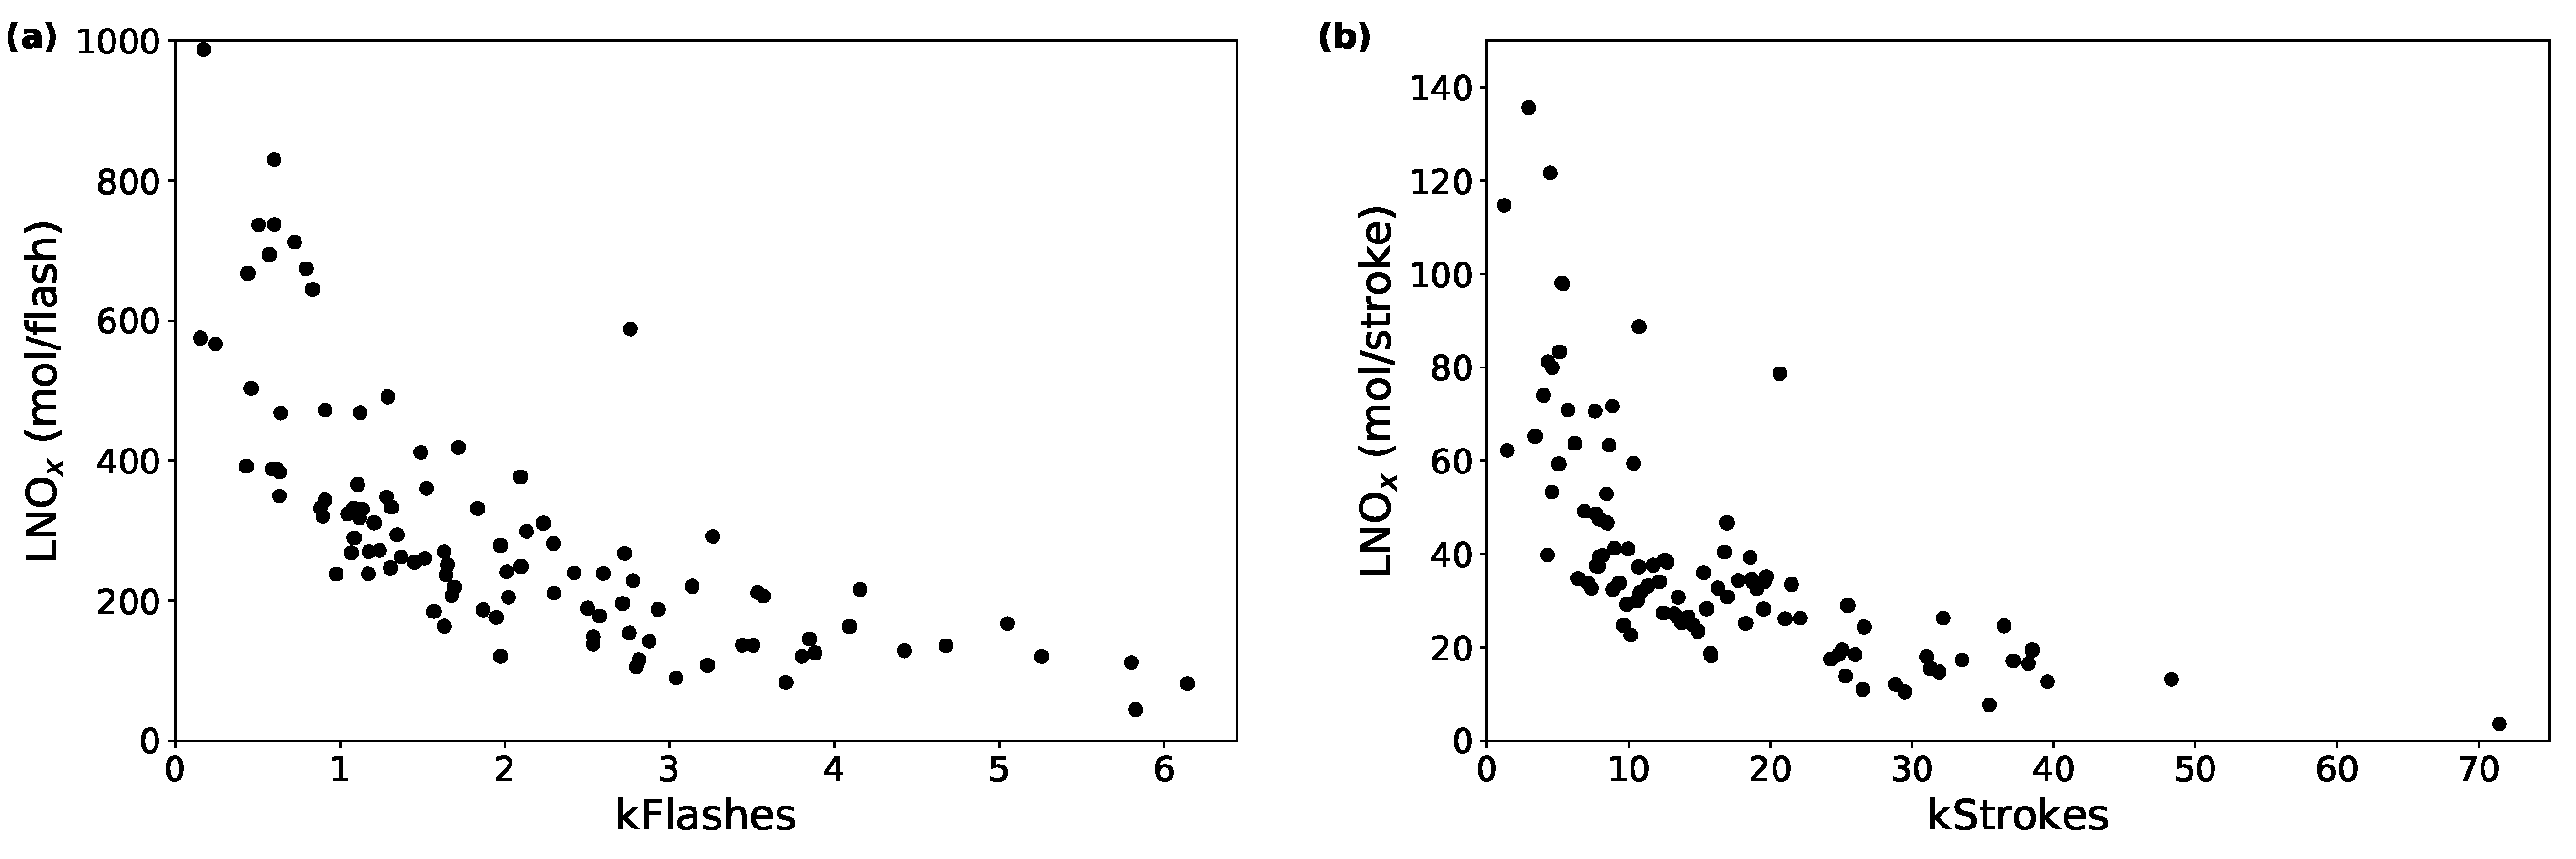
\includegraphics[width=15cm]{./figures/flash_threshold.pdf}
    \caption{
    (a) 每日 LNO$_x$ 产率与 ENTLN 总闪的关系,筛选条件为CRF $\geq$ 90\% 且1$^{\circ}$ $\times$ 1$^{\circ}$网格中至少有1次闪电。
     (b) 与 (a) 相同,但针对闪击。\\
    Figure \ref{fig:flash_threshold}. (a) Daily LNO$_\textrm{x}$ production efficiencies versus ENTLN total flashes data, with CRF $\geq$ 90\% and a flash threshold of 1 flash box$^{-1}$.
    (b) Same as (a) but for strokes.}
    \label{fig:flash_threshold}
\end{figure}


为确保WRF-Chem成功模拟闪电并考虑到闪电参数化的不确定性,我们将每个1$^{\circ}$ $\times$ 1$^{\circ}$网格模拟的总闪电(TL)阈值设置为1000,该阈值低于ENTLN闪电观测使用的阈值。
针对除LNO$_2$之外的其他NO$_2$源,我们定义了模拟的云上闪电NO$_2$柱密度(LNO$_2$Vis)与云上NO$_2$柱密度(NO$_2$Vis)之比,来判断OMI是否可以检测到足够的LNO$_2$。
该比率$\geq$50\%表明云层上方超过一半的NO$_x$具有LNO$_x$源。
此外,还需考虑氧化有关的NO$_2$寿命。
\citet{Nault.2017}的研究表明NO$_2$在对流附近的寿命($\tau$)为$\approx$3 h,故NO$_2$的初始值可由方程式(\ref{eq:inition})求解。

\begin{equation} \label{eq:inition}
NO_2(0) = NO_2(OMI) \times e^{0.5t/\tau}
\end{equation}

其中$NO_2(0)$是在时间 t=0 排放的NO$_2$摩尔数,$NO_2(OMI)$是在 OMI 过境时间测得的NO$_2$摩尔数,
0.5t是穿过网格的时间,即1.2 h,(假设闪电出现在每个1$^{\circ}$ $\times$ 1$^{\circ}$网格的中心)。
每个网格的V$_\textrm{LNO$_x$}$为网格中所有0.05$^{\circ}$ $\times$ 0.05$^{\circ}$像素的V$_\textrm{LNO$_x$}$平均值,
然后乘以网格的面积得到LNO$_x$摩尔数。

最后,有两种方法可用于估算季节性平均LNO$_2$每闪电、LNO$_x$每闪电、LNO$_x$每闪击和 LNO$_x$每闪击:

(1)求和法,将LNO$_x$的总和除以5--8月中每个1$^{\circ}$ $\times$ 1$^{\circ}$网格里发生的闪电或闪击总数;

(2)线性回归方法,将线性回归应用于LNO$_x$和每日闪电或闪击的平均值。

\subsection{适合反演闪电氮氧化物的条件} \label{subsec:criteria}

根据上节定义的条件,我们定义了六种不同的筛选条件组合(表),并使用线性回归方法(表)应用于原始数据。

\begin{table*}[h]
\scriptsize
\caption{本研究中使用的标准的缩写定义\\Table \ref{table:Abbreviations}Definitions of the abbreviations for the criteria used in this study.}
\begin{tabular}{ll}
\hline
\textbf{缩写} & \textbf{全称 [来源]} \\
\hline
CRF                             & Cloud radiance fraction [OMI] \\
CP                              & Cloud optical pressure [OMI] \\
CF                              & Cloud fraction [WRF-Chem] \\
TL                              & Total lightning flashes [WRF-Chem] \\
ratio                           & modeled LNO$_2$Vis / modeled NO$_2$Vis [WRF-Chem] \\
CRF$\alpha$\_ENTLN                    & CRF $\geq$ $\alpha$ + ENTLN flashes(strokes) $\geq$ 2400(8160) [ENTLN]\\
CRF$\alpha$\_CF40\_ENTLN              & CRF $\geq$ $\alpha$ + ENTLN flashes(strokes) $\geq$ 2400(8160) + CF $\geq$ 40\% \\
CRF$\alpha$\_ENTLN\_TL1000            & CRF $\geq$ $\alpha$ + ENTLN flashes(strokes) $\geq$ 2400(8160) + TL $\geq$ 1000 \\
CRF$\alpha$\_CF40\_ENTLN\_TL1000      & CRF $\geq$ $\alpha$ + ENTLN flashes(strokes) $\geq$ 2400(8160) + CF $\geq$ 40\% + TL $\geq$ 1000 \\
CRF$\alpha$\_ENTLN\_TL1000\_ratio50   & CRF $\geq$ $\alpha$ + ENTLN flashes(strokes) $\geq$ 2400(8160) + TL $\geq$ 1000 + ratio $\geq$ 50\% \\
CRF$\alpha$\_CF40\_ENTLN\_TL1000\_ratio50 & CRF $\geq$ $\alpha$ + ENTLN flashes(strokes) $\geq$ 2400(8160) + CF $\geq$ 40\% + TL $\geq$ 1000 + ratio $\geq$ 50\% \\
CRF$\alpha$\_ENTLN1(3.4)\_TL1\_ratio50    & CRF $\geq$ $\alpha$ + ENTLN flashes(strokes) $\geq$ 1(3.4) + TL $\geq$ 1 + ratio $\geq$ 50\% \\
\hline
\multicolumn{2}{l}{$^{*}$$\alpha$有三种选择:70\%、90\%以及100\%} \\
\multicolumn{2}{l}{$^{*}$$\alpha$ has three options: 70\%, 90\% and 100\%}
\end{tabular}
\label{table:Abbreviations}
\end{table*}


\begin{table*}[h]
\scriptsize
\caption{根据表\ref{table:Abbreviations}中的定义得到的LNO$_\textrm{x}$产率\\Table \ref{table:conditions} LNO$_\textrm{x}$ production efficiencies for different combinations of criteria defined in Table \ref{table:Abbreviations}.}
\begin{tabular}{lccccc}
\hline
\textbf{条件$^1$} & \textbf{ENTLN类型$^2$} & \textbf{LNO$_\textrm{x}$/flash or LNO$_\textrm{x}$/stroke} & \textbf{R值} & \textbf{截距 (10$^{6}$mol)} & \textbf{天数$^3$} \\
\hline
CRF90\_ENTLN                        & Flash  & 52.1 $\pm$ 51.1 & 0.20 & 0.21  & 99 \\
CRF90\_CF40\_ENTLN                  & Flash  & 84.2 $\pm$ 31.5 & 0.54 & -0.04 & 70 \\
CRF90\_ENTLN\_TL1000                & Flash  & 61.9 $\pm$ 49.1 & 0.27 & 0.33  & 83 \\
CRF90\_CF40\_ENTLN\_TL1000          & Flash  & 63.4 $\pm$ 52.9 & 0.38 & 0.26  & 38 \\
CRF90\_ENTLN\_TL1000\_ratio50       & Flash  & 54.5 $\pm$ 48.1 & 0.25 & 0.39  & 81 \\
CRF90\_CF40\_ENTLN\_TL1000\_ratio50 & Flash  & 90.0 $\pm$ 65.0 & 0.46 & 0.15  & 32 \\
CRF90\_ENTLN                        & Stroke & 6.7 $\pm$ 4.1 & 0.31 & 0.23  & 102 \\
CRF90\_CF40\_ENTLN                  & Stroke & 10.3 $\pm$ 3.6 & 0.55 & 0.08 & 79 \\
CRF90\_ENTLN\_TL1000                & Stroke & 7.5 $\pm$ 5.1 & 0.29 & 0.38  & 94 \\
CRF90\_CF40\_ENTLN\_TL1000          & Stroke & 8.6 $\pm$ 6.2 & 0.39 & 0.27  & 46 \\
CRF90\_ENTLN\_TL1000\_ratio50       & Stroke & 7.0 $\pm$ 4.8 & 0.29 & 0.42  & 93 \\
CRF90\_CF40\_ENTLN\_TL1000\_ratio50 & Stroke & 8.9 $\pm$ 7.0 & 0.39 & 0.31  & 40 \\
\hline
\multicolumn{6}{l}{$^1$定义见表\ref{table:Abbreviations}。}\\
\multicolumn{6}{l}{$^2$ENTLN阈值为OMI过境前2.4小时内,1$^{\circ}$ $\times$ 1$^{\circ}$网格中闪电至少2400次和闪击至少8160次。}\\
\multicolumn{6}{l}{$^3$2014年5--8月中有效的天数。} \\
\multicolumn{6}{l}{$^1$These conditions are defined in Table \ref{table:Abbreviations}.} \\
\multicolumn{6}{l}{$^2$The thresholds of ENTLN data are 2400 flashes box$^{-1}$ and 8160 strokes box$^{-1}$ during the period of 2.4 h before OMI overpass time.} \\
\multicolumn{6}{l}{$^3$The number of valid days with specific criteria in MJJA 2014.}
\label{table:conditions}
\end{tabular}
\end{table*}


在CRF90\_ENTLN条件下,有效闪电(闪击)数据对应共有99(102)天。
以闪电类ENTLN数据为例,在 CRF90\_ENTLN\_TL1000\_ratio50 条件下,有效天数从 99 减少至 81,而LNO$_x$产率从 52.1$\pm$51.1 mol每闪电增加到 54.5$\pm$48.1 mol每闪电。
该结果与 CRF90\_ENTLN\_TL1000 条件下所得的结果几乎相同。
尽管这表明TL筛选条件已足够严格,但最好包括云上LNO$_2$占比的筛选条件,以防不同的AMF方法中存在一些例外情况。
由于 CF $\geq$ 40\% 会导致有效数据和产率急剧下降,因此我们仅仅使用 CRF 对数据进行筛选。
最后,我们选择至少2400次闪电或至少8160次闪击,TL $\geq$ 1000 和云上LNO$_2$占比 $\geq$ 50\% 作为阈值,来探索三种不同 CRF 条件(CRF $\geq$ 70\%、CRF $\geq$ 90\% 和 CRF = 100\%)对 LNO$_x$ 估算产生的影响(表\ref{table:CRFs})。
当CRF 标准从 70\% 增加到 90\% 和 100\%时,针对闪电类型的LNO$_x$产率 从35.7$\pm$36.8 mol每闪电增加到 54.5$\pm$48.1 mol每闪电,然后再降低到20.8$\pm$37.4 mol每闪电,而针对闪击类型的LNO$_x$产率从4.1$\pm$3.9 mol每闪击提高到 7.0$\pm$4.8 mol每闪击,然后再次下降到2.6$\pm$4.0 mol每闪击(表\ref{table:CRFs})。
当 CRF 从 90\% 增加到 100\% 时LNO$_x$ PE 降低,这是因为闪电密度较高而 LNO$_x$ 较少。
CRF 从 70\% 增加到 90\% 引起的 LNO$_x$ PE 增加与\citet{Pickering.2016}的结果相反。
这是由于我们的方法中考虑了从边界层传输的 NO$_2$ 污染的影响。
虽然在 CRF > 70\% 的地区经常观察到 NO$_x$ 增强\citet{Pickering.2016},但考虑到中低浓度 NO$_2$ 的污染并与\citet{Pickering.2016}和\citet{Lapierre.2020}的结果进行比较,以下分析将基于 CRF $\geq$ 90\% 标准进行讨论分析。

\begin{table*}[h]
\scriptsize
\caption{在相同ENTLN阈值,TL $\geq$ 1000 和云上LNO$_2$占比 $\geq$ 50\%的条件下,不同云辐射分数阈值对应的LNO$_\textrm{x}$产率 \\ LNO$_\textrm{x}$ production efficiencies for different thresholds of CRF with coincident ENTLN data, TL $\geq$ 1000 and ratio $\geq$ 50\%.}
\begin{tabular}{cccccc}
\hline
\textbf{云辐射分数 (\%)} & \textbf{ENTLN类型$^1$} & \textbf{LNO$_\textrm{x}$每闪电 or LNO$_\textrm{x}$每闪击} & \textbf{R值} & \textbf{截距 (10$^{5}$mol)} & \textbf{天数$^2$} \\
\hline
70  & 闪电  & 35.7  $\pm$ 36.8 & 0.21 & 4.91 & 85 \\
90  & 闪电  & 54.5  $\pm$ 48.1 & 0.25 & 3.90 & 81 \\
100 & 闪电  & 20.8  $\pm$ 37.4 & 0.13 & 5.67 & 71 \\
70  & 闪击 & 4.1   $\pm$ 3.9  & 0.21 & 5.16 & 96 \\
90  & 闪击 & 7.0   $\pm$ 4.8  & 0.29 & 4.16 & 93 \\
100 & 闪击 & 2.6   $\pm$ 4.0  & 0.14 & 5.41 & 82 \\
\hline
\multicolumn{6}{l}{$^1$ENTLN阈值为 OMI f过境前 2.4 小时内每个网格闪电至少 2400 次 或 闪击至少8160 次。}\\
\multicolumn{6}{l}{$^2$2014年5--8月对应筛选条件下有效天数。} \\
\multicolumn{6}{l}{$^1$The thresholds of ENTLN data are 2400 flashes box$^{-1}$ and 8160 strokes box$^{-1}$ during the period of 2.4 h before OMI overpass time.}\\
\multicolumn{6}{l}{$^2$The number of valid days with specific criteria in MJJA 2014.}
\end{tabular}
\label{table:CRFs}
\end{table*}

\subsection{不同反演方法的对比}

\citet{Lapierre.2020}基于 BEHR NO$_2$ 产品得出 LNO$_2$ 产量,
为了使本研究的结果与\citet{Pickering.2016}和\citet{Lapierre.2020}的结果具有可比性,我们选择 NO$_2$  而不是 NO$_x$  来计算每次闪电的产量(产率,PE)。
在图\ref{fig:pe_timeseries}中,根据 CRF $\geq$ 90\% 和每 2.4 h 2400次闪电的阈值,绘制了2014年5--8月美国大陆每天 NO$_2$Vis、LNO$_2$Vis、LNO$_2$ 和 LNO$_2$Clean 产率的时间序列图。
其中,LNO$_2$ PE 大多在 20 至 80 mol每闪电的范围内,LNO$_2$Vis PE 小于 LNO$_2$ PE,因为后者在云层下含有 LNO$_2$。
\citet{Pickering.2016}的GMI模拟结果表明,25\%--30\%的LNO$_x$柱密度位于 云压(CP)以下,而我们的 WRF-Chem 模拟结果显示该比例为 56$\pm$20\%。
云属性对 LNO$_x$ PE 的影响将在第\ref{susbec:china_uncertainty}节中进行更详细地讨论。
总体而言,估算得到的每日PE顺序为LNO$_2$Clean > LNO$_2$ > NO$_2$Vis > LNO$_2$Vis。
通过NO$_2$Vis 和 LNO$_2$Vis 估算得到的PE之间的差异($\Delta$PE)表明有一定量的背景 NO$_2$ 存在于云层之上。
总体而言,该 $\Delta$PE 的趋势与 NO$_2$Vis 和 LNO$_2$Clean 之间的$\Delta$PE 一致。
当区域污染严重时(NO$_2$Vis 和 LNO$_2$Vis 之间的 $\Delta$PE > 200\%),基于 NO$_2$Vis 和 LNO$_2$Clean 的 PE 被显著高估。
换言之,NO$_2$Vis 和 LNO$_2$Clean 对背景 NO$_2$ 更为敏感。
且在高污染地区,NO$_2$Vis 的高估程度大于 LNO$_2$Clean,而在其他大多数地区通常相反。

\begin{figure}[h]
\centering
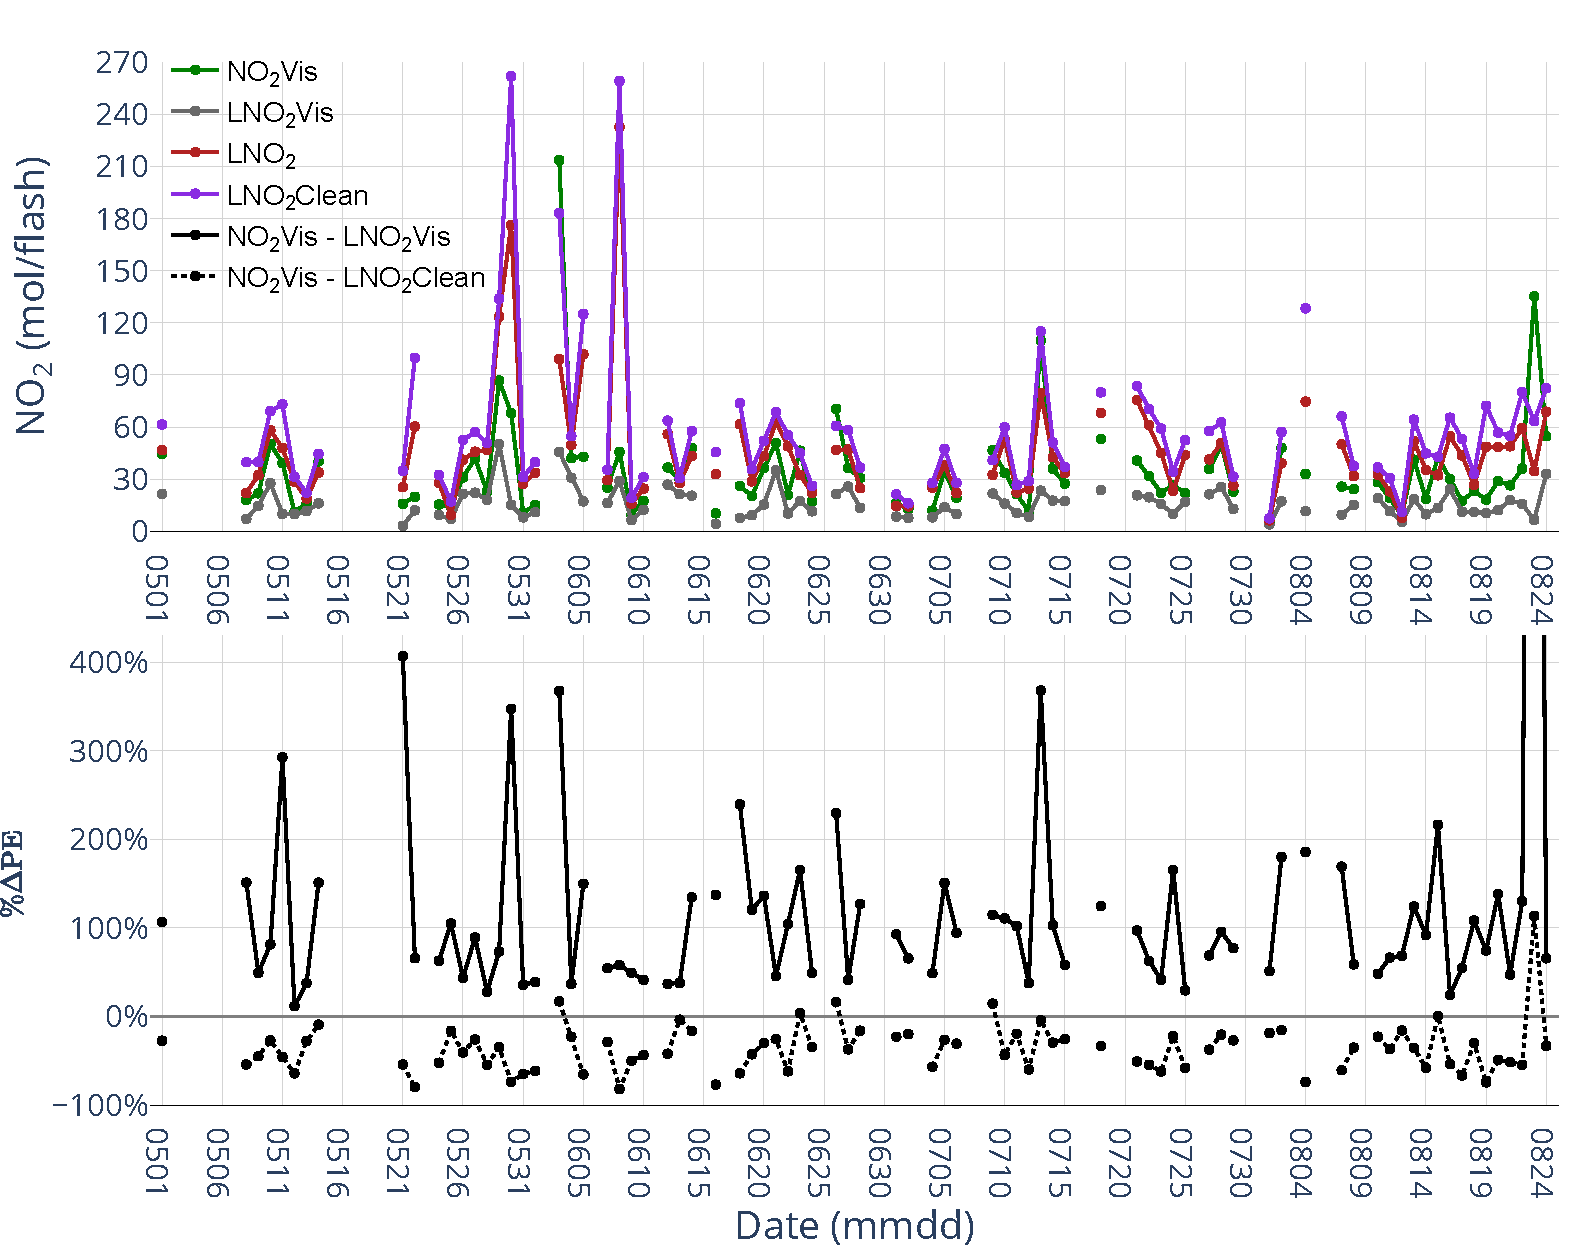
\includegraphics[width=12cm]{./figures/pe_timeseries.pdf}
\caption{(上图)NO$_2$Vis、LNO$_2$Vis、LNO$_2$ 和 LNO$_2$Clean产率的时间序列(2014年5--8月美国大陆),筛选条件为CRF $\geq$ 90\% 和每 2.4 小时 至少2400 次闪电。
(下图)在CRF$\geq$ 90\%的条件下,NO$_2$Vis 和 LNO$_2$Vis 之间百分比差异以及 NO$_2$Vis 和 LNO$_2$Clean 之间百分比差异的时间序列。
8 月 23 日黑点的值(未显示)为 1958\%。\\
Figure \ref{fig:pe_timeseries}. (top) Time series of NO$_2$Vis, LNO$_2$Vis, LNO$_2$ and LNO$_2$Clean production per day over the CONUS for MJJA 2014 with CRF $\geq$ 90\% and a flash threshold of 2400 flashes per 2.4 h.
(bottom) Time series of the percent differences between NO$_2$Vis and LNO$_2$Vis and the percent differences between NO$_2$Vis and LNO$_2$Clean with CRF $\geq$ 90\%.
The value of black dot on August 23 (not shown) is 1958\%.}
\label{fig:pe_timeseries}
\end{figure}

如图\ref{fig:pe_linear}所示,ENTLN 数据与 NO$_2$Vis、LNO$_2$Vis、LNO$_2$ 和 LNO$_2$Clean的线性回归,其筛选条件与图 \ref{fig:pe_timeseries} 相同。
LNO$_2$Clean PE为 25.2$\pm$22.3 mol NO$_2$ 每闪电,相关系数为 0.25 和 2.3$\pm$2.1 mol NO$_2$每闪击,相关系数为 0.22。
如图\ref{fig:pe_timeseries}所示,NO$_2$Vis PE 和 LNO$_2$Clean PE 之间的正百分比差异发生的频率远低于负差异的发生频率。
因此,NO$_2$Vis PE(17.1$\pm$17.2 mol NO$_2$ 每闪电和0.4$\pm$1.0 mol NO$_2$ 每闪击)小于使用线性回归方法得到的 LNO$_2$Clean PE。

\begin{figure}[t]
    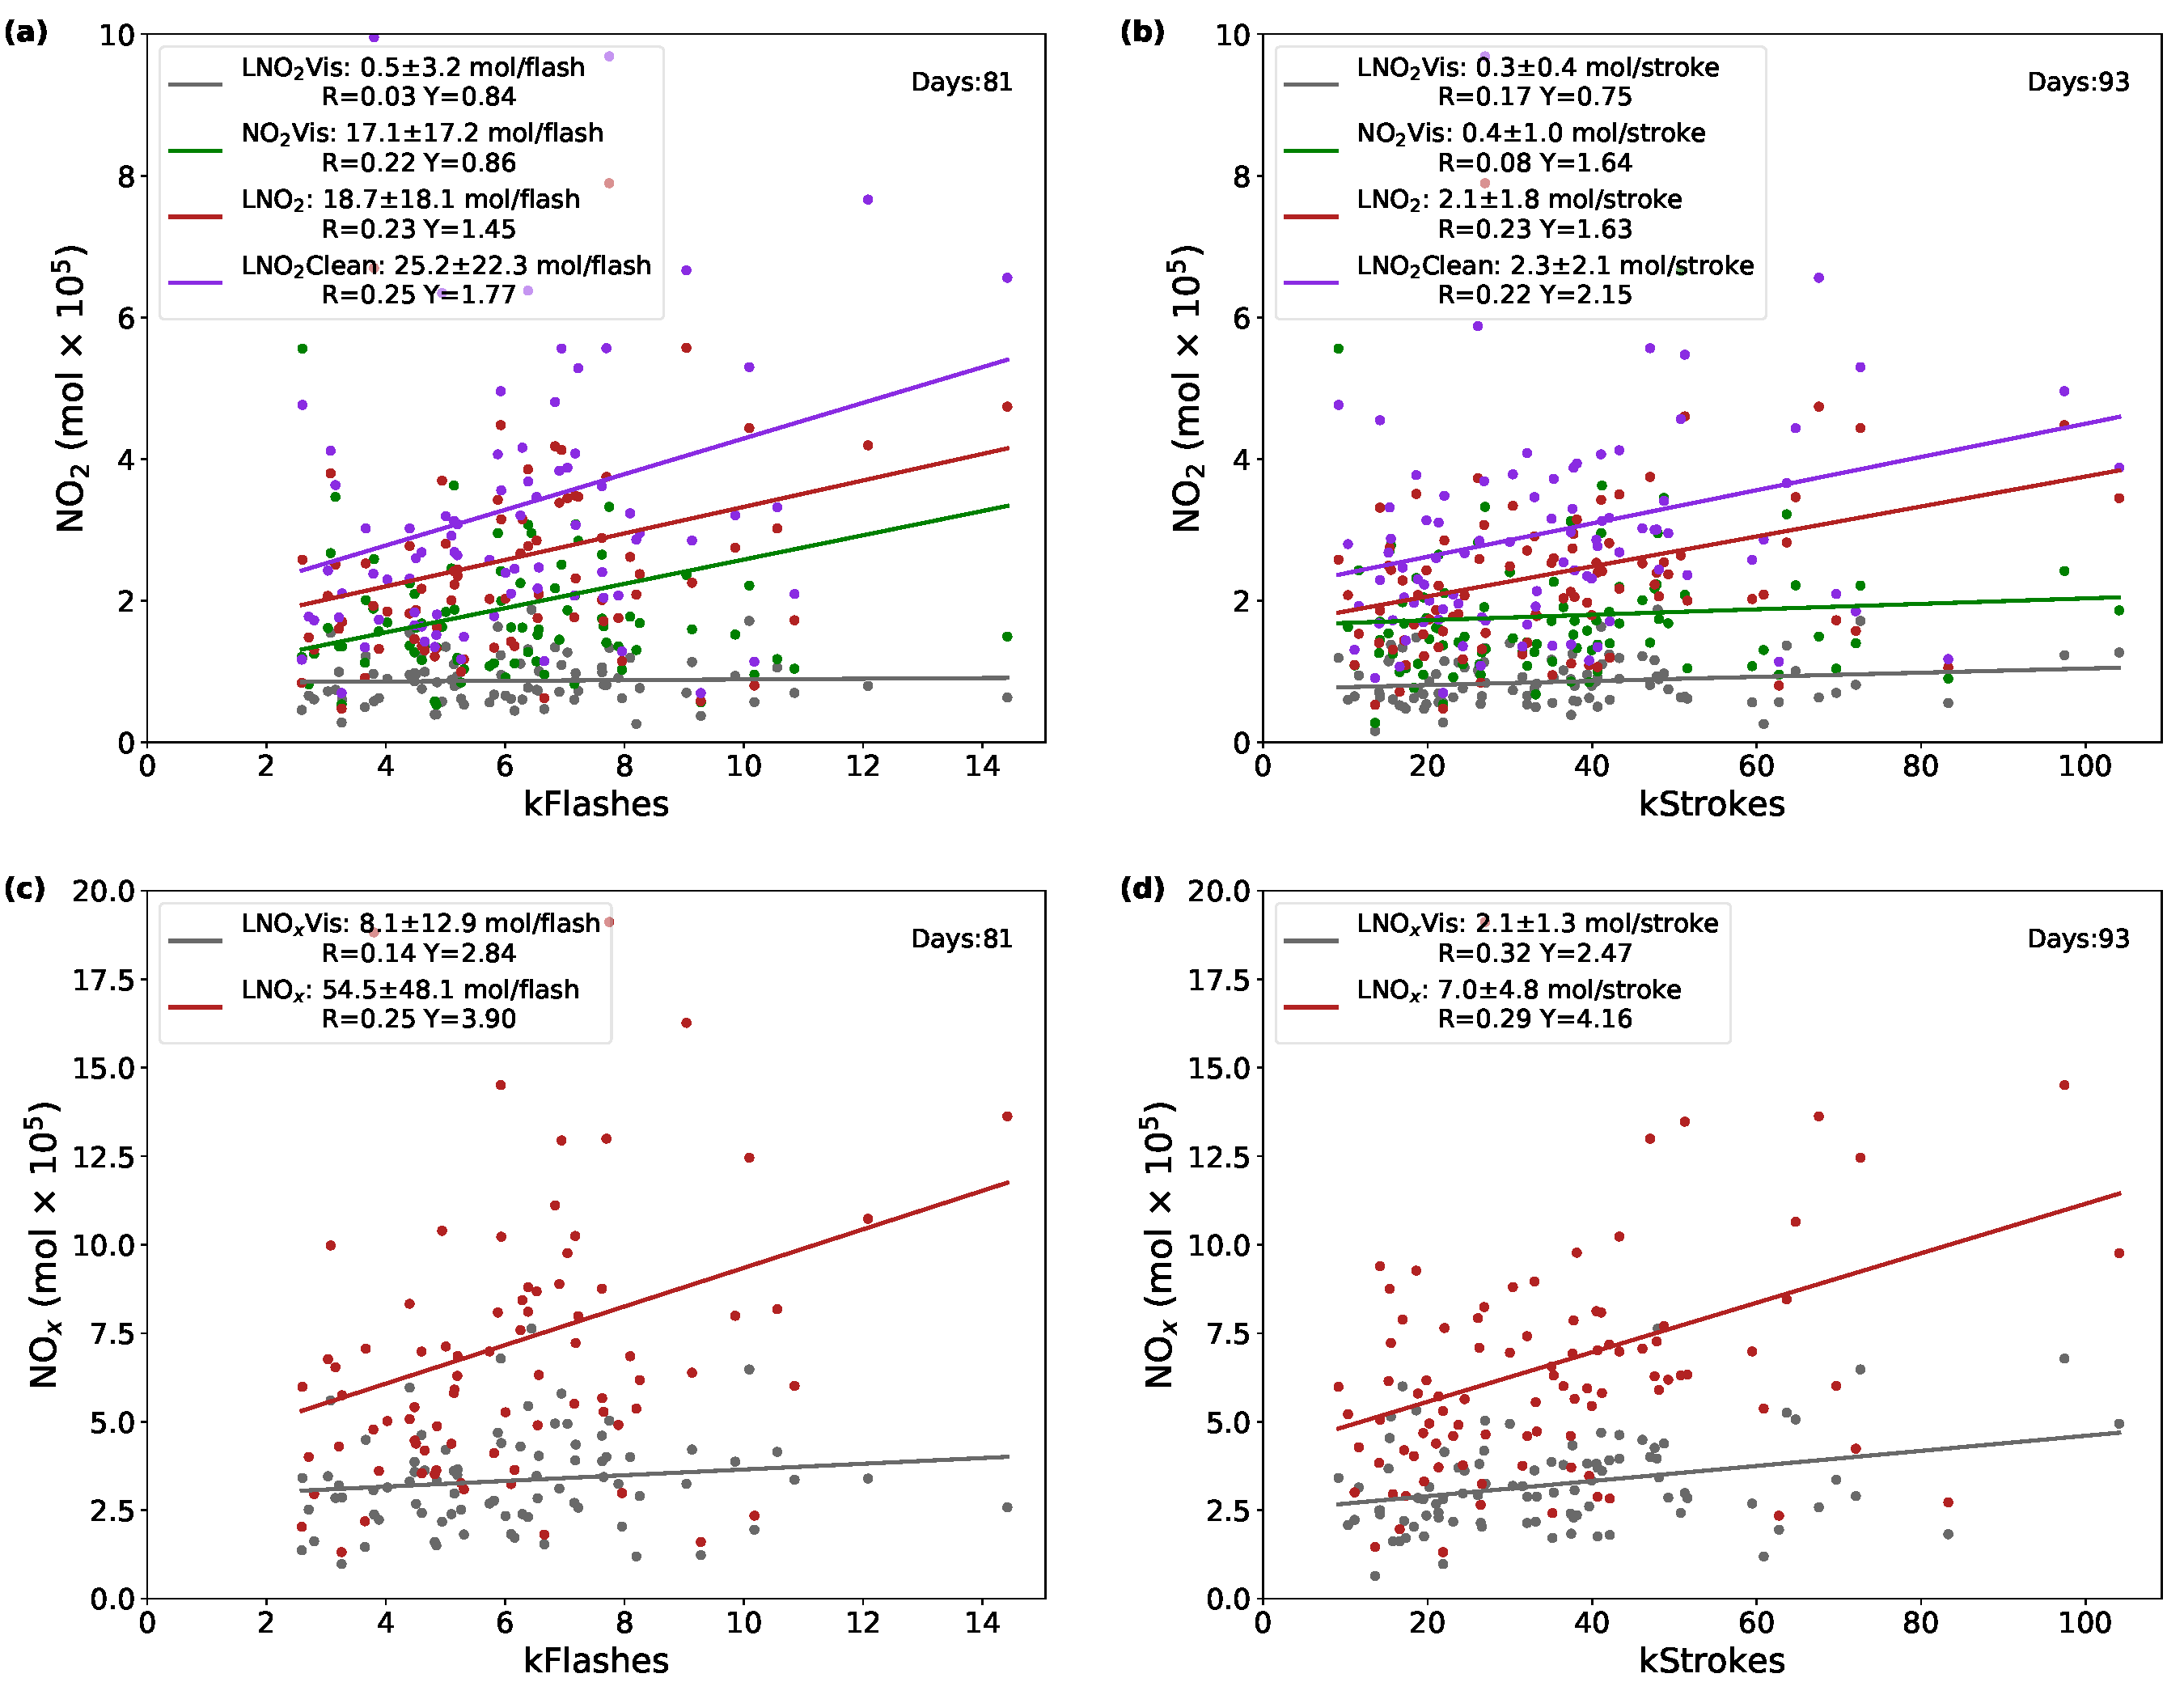
\includegraphics[width=15cm]{./figures/pe_linear.pdf}
    \caption{(a) 每日 NO$_2$Vis、LNO$_2$Vis、LNO$_2$ 和 LNO$_2$Clean 与 ENTLN 总闪的关系。
    (b) 与 (a) 相同,但针对闪击数据。
    (c) 每日 LNO$_x$Vis 和 LNO$_x$ 与总闪的关系。
    (d) 与 (c) 相同,但针对闪击数据。\\
    Figure \ref{fig:pe_linear}. (a) Daily NO$_2$Vis, LNO$_2$Vis, LNO$_2$ and LNO$_2$Clean versus ENTLN total flashes data.
    (b) Same as (a) but for strokes. (c) Daily LNO$_x$Vis and LNO$_x$ versus total flashes. (d) Same as (c) but for strokes.}
    \label{fig:pe_linear}
\end{figure}

为了将我们的结果与\citet{Lapierre.2020}的结果进行比较,
我们从筛选条件中取出CP $\leq$ 650 hPa、TL $\geq$ 1000 和 ratio $\geq$ 50 \% 的条件。
但是,我们得到的NO$_2$Vis(3.8$\pm$0.5 mol每闪击)仍大于\citet{Lapierre.2020}的1.6$\pm$0.1 mol每闪击。
这可能是由两者使用不同版本的伯克利高分辨率(BEHR)算法引起的,\citet{Lapierre.2020}使用的是BEHR v3.0A,我们的算法基于BEHR v3.0B \citep{Laughner.2019a}。
两个版本中S$_{\textrm{NO$_2$}}$均来自于NASA标准产品v3,BEHR v3.0B 的主要改进如下:

(1)使用最接近 OMI 过境时间的廓线,而不是 OMI 过境之前的最后一个时刻的廓线;

(2)AMF 使用可变的对流层顶高度,而不是固定的200 hPa 对流层顶;

(3)根据\citet{Zhou.2009}的方法计算地表气压。

详细的更新日志见\url{https://github.com/CohenBerkeleyLab/BEHR-core/blob/master/Documentation/Changelog.txt}。
此外,\citet{Lapierre.2020}使用了月平均NO$_2$廓线,而我们的研究使用了日廓线,并且我们将WRF-Chem 输出的间隔调整为 30 min,
这比BEHR 每日产品(1 h)输出间隔更短,但 AMF 可能会受到不同 NO$_2$ 剖面的影响。
鉴于这些因素,我们在所得数据的基础上来比较不同的方法,以尽量减少这些影响。

同时,LNO$_2$ PE(18.7$\pm$18.1 mol每闪电,2.1$\pm$1.8 mol每闪击)介于 LNO$_2$Clean PE 和 NO$_2$Vis PE 之间,与图 \ref{fig:pe_timeseries} 中的日结果一致。
此外,基于每日LNO$_x$ PE 求和值的线性回归结果为114.8$\pm$18.2 mol每闪电(或17.8$\pm$2.9 mol每闪击),该结果大于\citet{Pickering.2016}的91 mol每闪电。
这一差异可能是由地理位置、闪电数据和化学模型所共同导致的。

在 CRF $\geq$ 90\% 下,LNO$_2$ PE 的平均值和标准差为 46.2$\pm$35.1 mol 每闪电和 9.9$\pm$8.1 mol 每闪电,
而 LNO$_x$ PE 为 125.6$\pm$95.9 mol 每闪电和 26.7$\pm$21.6 mol 每闪电(图\ref{fig:pe_sum})。
美国东南部的 LNO$_2$ PE 和 LNO$_x$ PE 均较高(由图\ref{fig:pe_sum}中的红框表示,25--37$^{\circ}$ N,75--95$^{\circ}$ W),这与\citet{Lapierre.2020} 和 \citet{Bucsela.2019}的研究结果相一致。
而与图\ref{fig:pe_timeseries}相比,图\ref{fig:delta}(a)和(b)显示NO$_2$Vis PE 和 LNO$_2$Vis PE 之间的一些较大差异,这与我们对污染区域的预期一致。
同时,LNO$_2$ PE 和 NO$_2$Vis PE 之间的差异取决于背景 NO$_2$、上升气流的强度和廓线分布。
负差异是由上升气流携带的背景 NO$_2$ 引起的,而云下 LNO$_2$ 的部分导致 LNO$_2$ PE 高于 NO$_2$Vis PE(图\ref{fig:delta}(c))。
图\ref{fig:delta}(d) 显示 LNO$_2$Vis 与 LNO$_2$占比为 10\%--80\%。
这可能是由云层的高度和 LNO$_2$ 的廓线造成的。
如果CP在300 hPa附近,由于云层的覆盖,该比值将更小。
因此,需要更好地了解LNO$_2$ 廓线和 云下的LNO$_x$。


\begin{figure}[h]
\centering
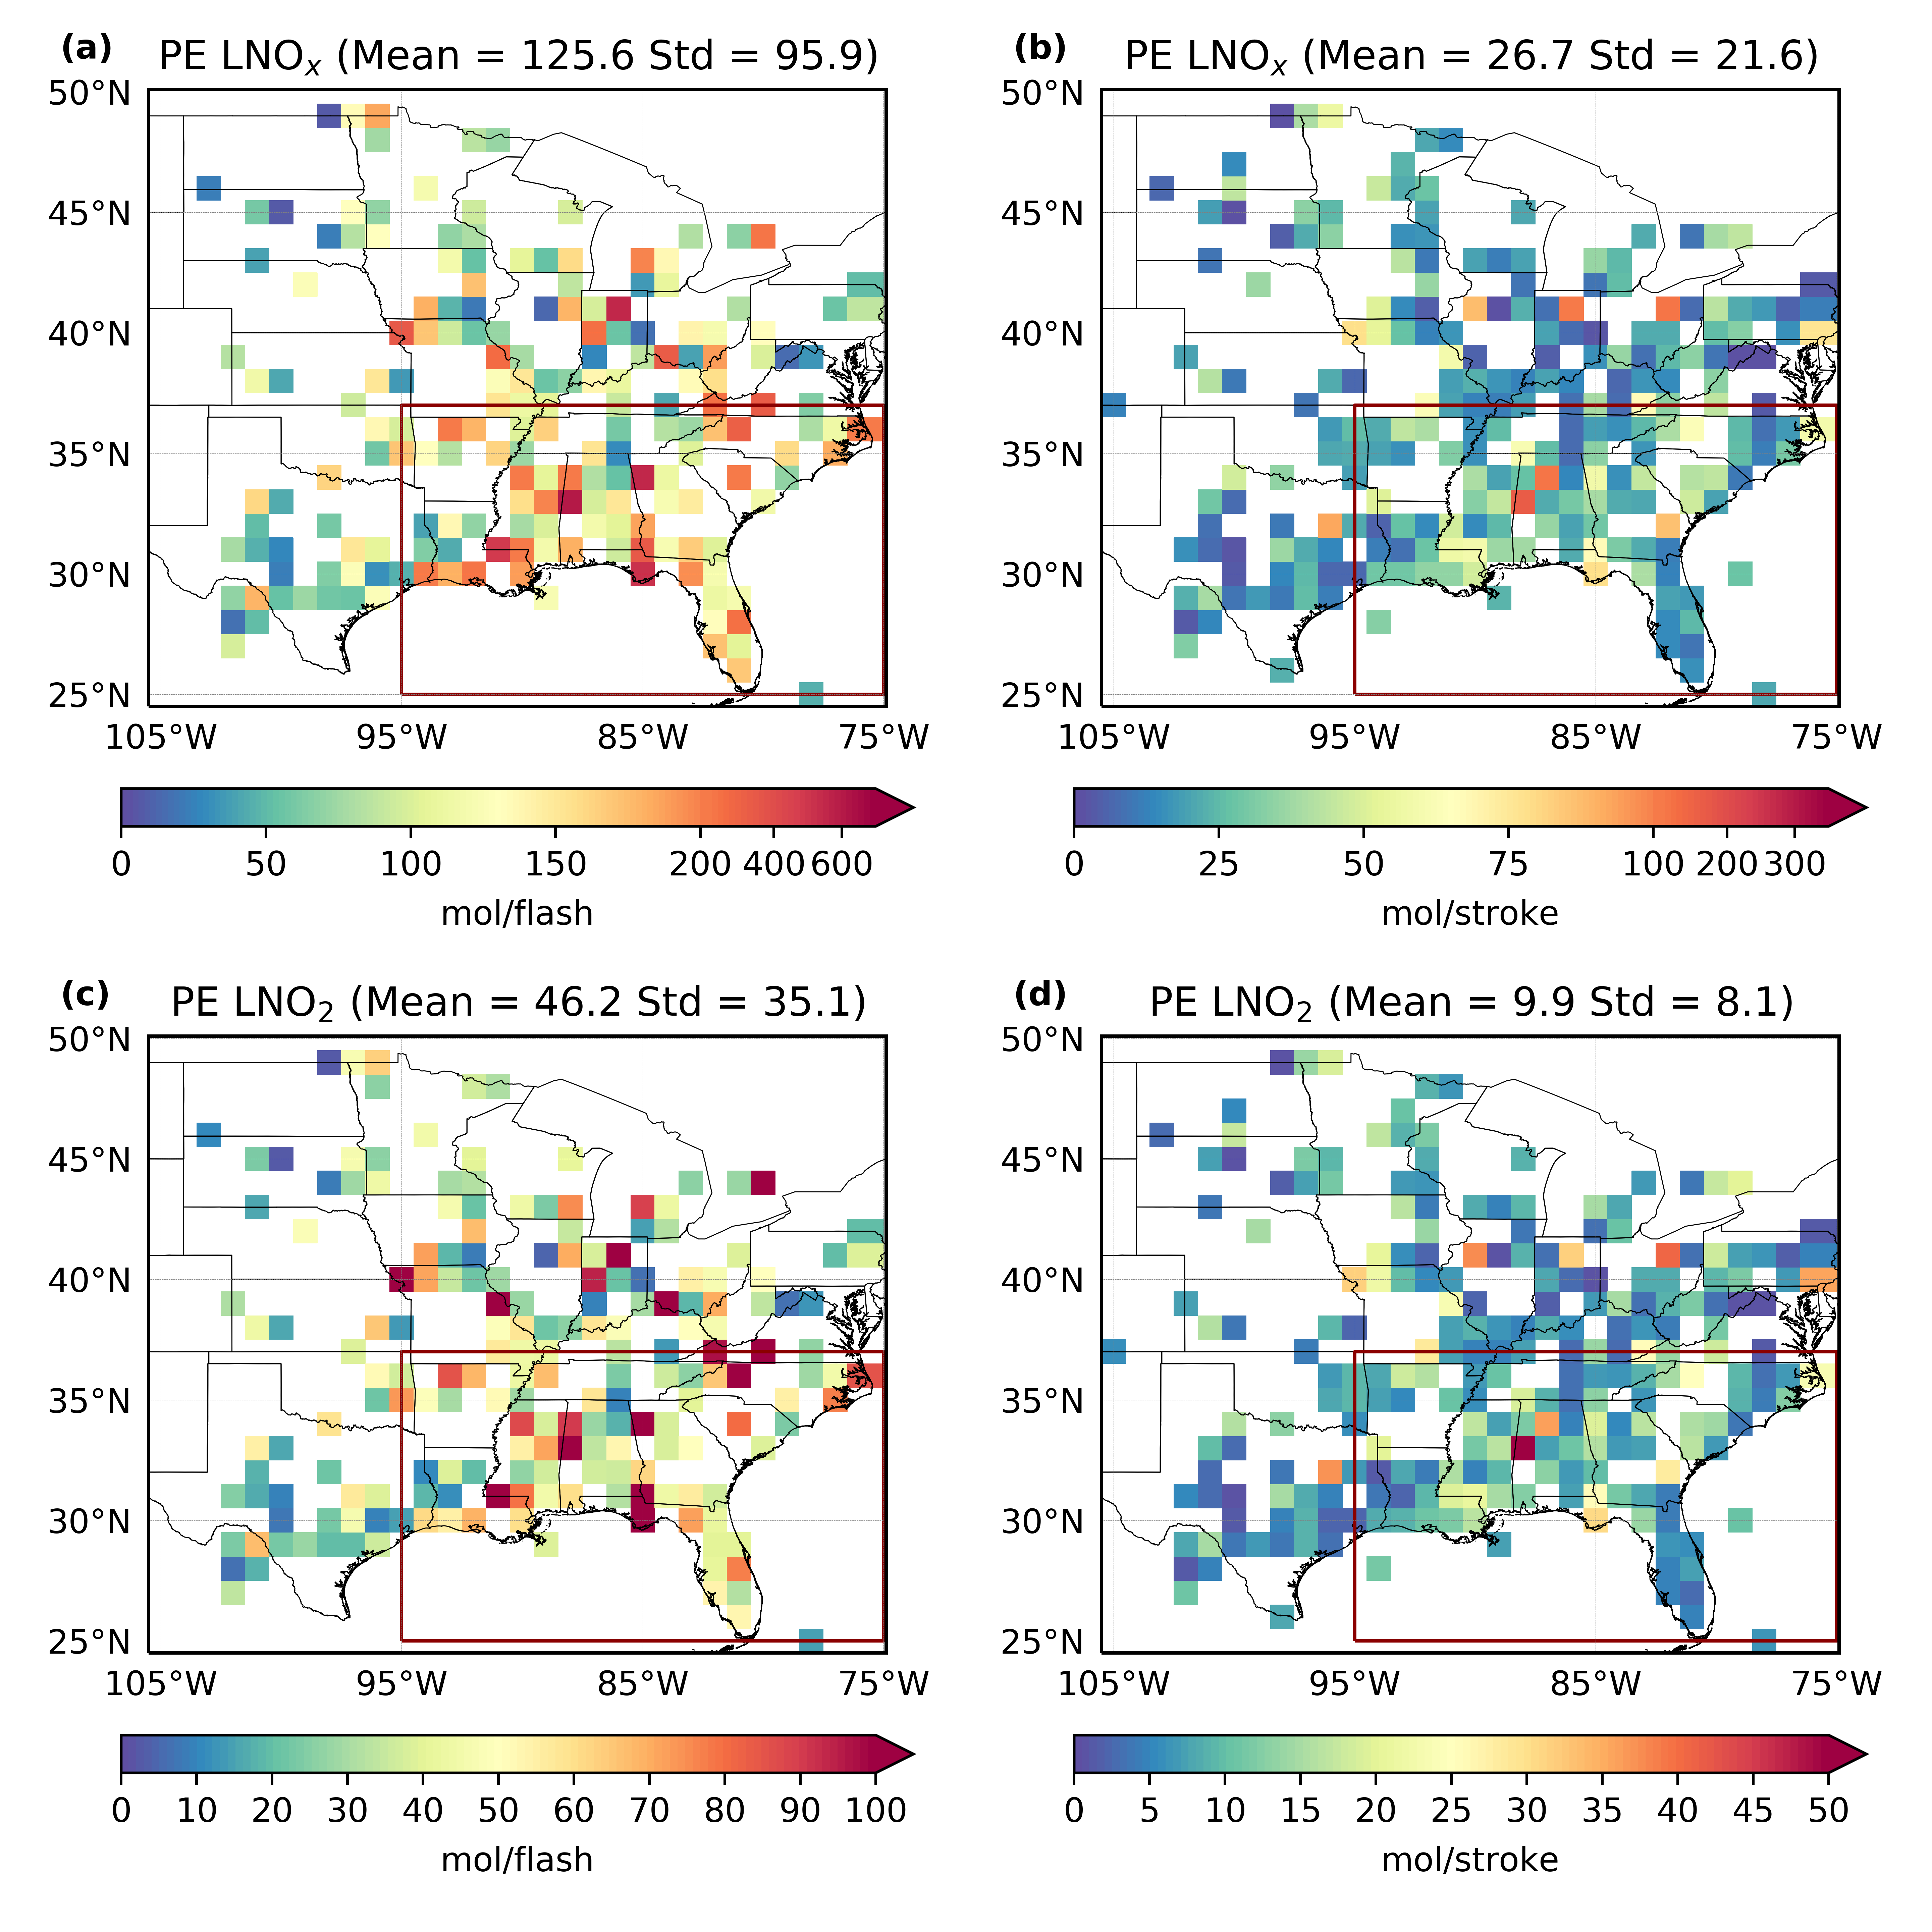
\includegraphics[width=13cm]{./figures/pe_sum.png}
\caption{(a) 和 (c) 在CRF $\geq$ 90\%条件下,2014年5--8月 1$^{\circ}$ $\times$ 1$^{\circ}$ LNO$_\textrm{x}$ 和LNO$_\textrm{2}$的平均产率分布图。
     (b) 和 (d) 与 (a) 和 (c) 相同,但针对闪击数据。美国东南部由红框表示。\\
     Figure \ref{fig:pe_sum}. (a) and (c) Maps of 1$^{\circ}$ $\times$ 1$^{\circ}$ gridded values of mean LNO$_\textrm{x}$
    and LNO$_\textrm{2}$ production per flash with CRF $\geq$ 90\% for MJJA 2014.
    (b) and (d) Same as (a) and (c) except for strokes.
    The southeastern US is denoted by the red box in panels a--d.
}
\label{fig:pe_sum}
\end{figure}

\begin{figure}[t]
\centering
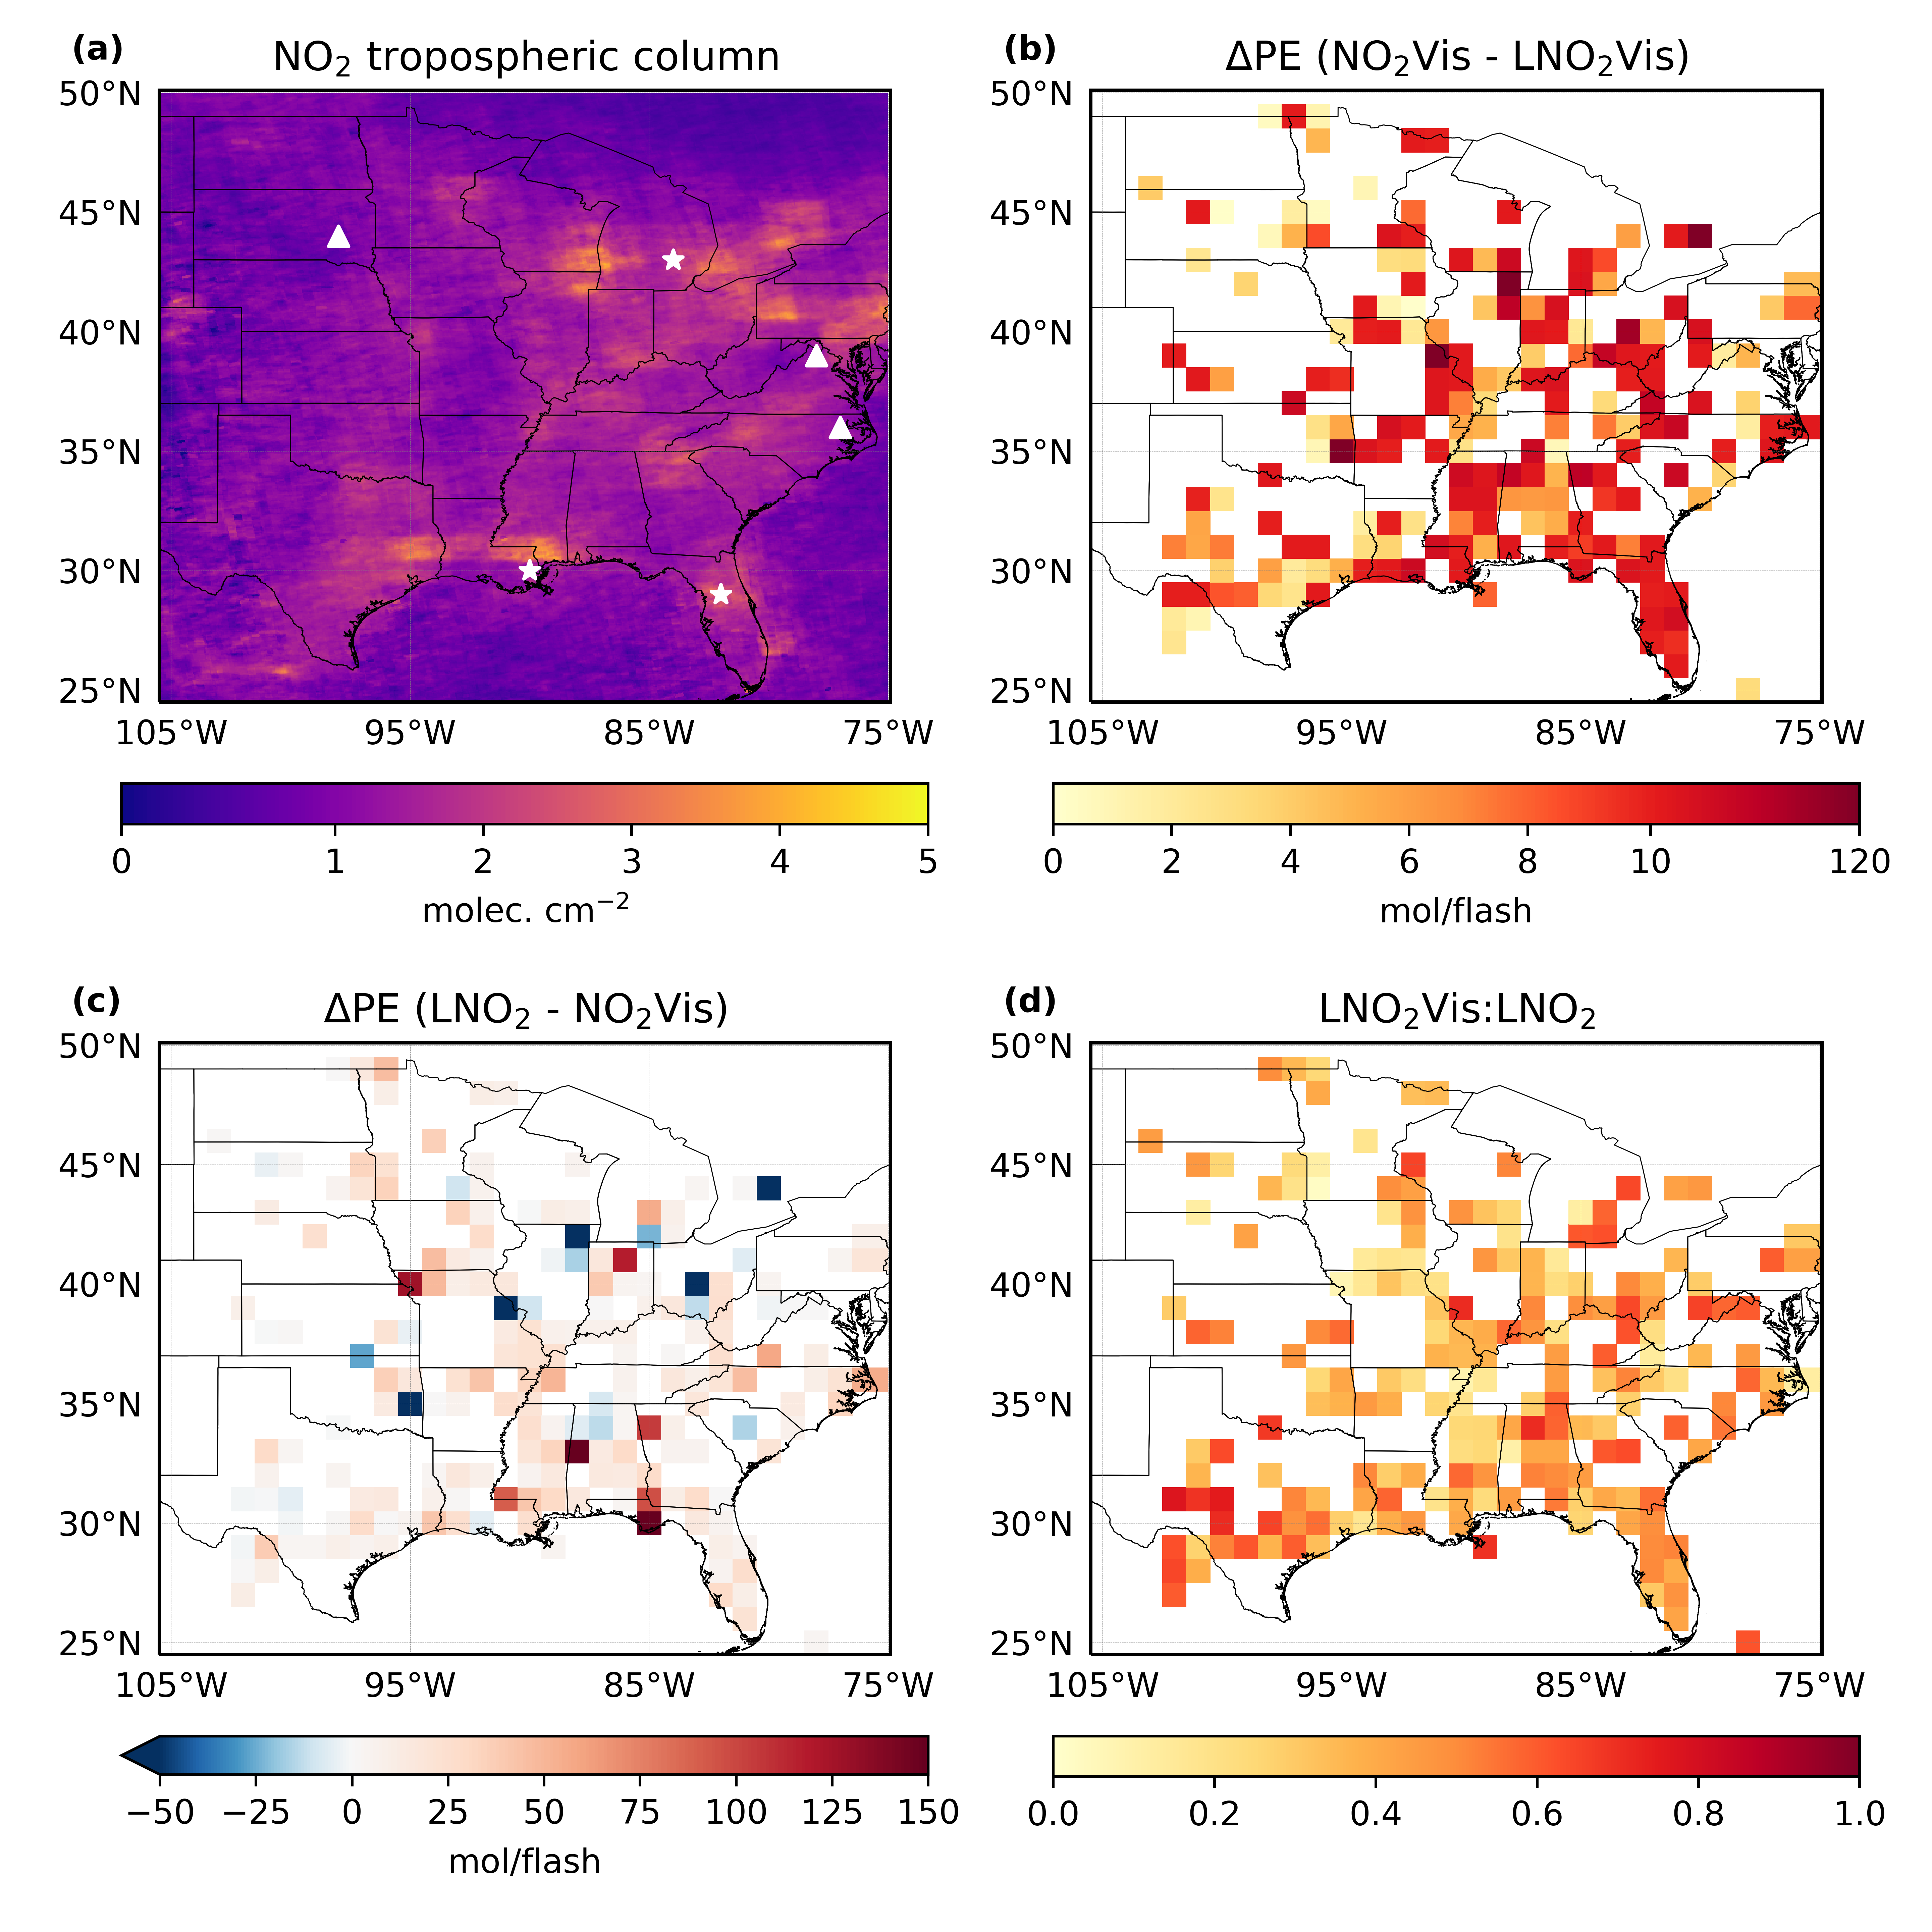
\includegraphics[width=13cm]{./figures/delta.png}
\caption{(a) 2014年5--8月  平均对流层NO$_\textrm{2}$柱浓度。
污染城市用星星表示:兰辛、新奥尔良和奥兰多,而清洁城市用三角形表示:休伦、查尔斯镇和塔伯勒。
(b) 在CRF $\geq$ 90\%条件下,NO$_\textrm{2}$Vis 和 LNO$_\textrm{2}$Vis平均产率的差异。
(c) 与 (b) 相同,但为 LNO$_\textrm{2}$ 和 NO$_\textrm{2}$Vis 之间的差异。
(d) LNO$_\textrm{2}$Vis 与 LNO$_\textrm{2}$ 的比例。\\
(a) Mean (MJJA 2014) NO$_\textrm{2}$ tropospheric column.
Polluted cities are denoted by stars: Lansing, New Orleans and Orlando while clean cities are denoted by triangles: Huron, Charles Town and Tarboro.
(b) The differences of the estimated mean production efficiency between NO$_\textrm{2}$Vis and LNO$_\textrm{2}$Vis with CRF $\geq$ 90\%.
(c) The same differences as (b) but between LNO$_\textrm{2}$ and NO$_\textrm{2}$Vis.
(d) The ratio of LNO$_\textrm{2}$Vis to LNO$_\textrm{2}$.
}
\label{fig:delta}
\end{figure}

\subsection{背景氮氧化物浓度和云属性对反演的影响}

鉴于图\ref{fig:delta}表明我们方法对于LNO$_2$产率估算的改进在污染和清洁地区是不同的。
为了简化量化,我们选择了CRF = 100\%条件下,具有相似云上NO$_2$廓线($\approx$ 100 pptv)的六个网格,这样AMF之间的差异取决于较少的参数。

\begin{equation} \label{AMFLNO2_crf100}
AMF_{\textrm{LNO$_2$}} = \frac{\int_{p_{\textrm cloud}}^{p_{\textrm tp}} w_{\textrm cloudy}(p) NO_2(p) \: dp}{\int_{p_{\textrm surf}}^{p_{\textrm tp}} LNO_2(p) \: dp}
\end{equation}

\begin{equation} \label{AMFNO2Vis_crf100}
AMF_{\textrm{NO$_2$Vis}} = \frac{\int_{p_{\textrm cloud}}^{p_{\textrm tp}} w_{\textrm cloudy}(p) NO_2(p) \: dp}{\int_{p_{\textrm cld}}^{p_{\textrm tp}} NO_2(p) \: dp}
\end{equation}

\begin{equation} \label{AMFLNO2Clean_crf100}
AMF_{\textrm{LNO$_2$Clean}} = \frac{\int_{p_{\textrm cloud}}^{p_{\textrm tp}} w_{\textrm cloudy}(p) LNO_2(p) \: dp}{\int_{p_{\textrm surf}}^{p_{\textrm tp}} LNO_2(p) \: dp}
\end{equation}

这些网格框分别包含图\ref{fig:delta}(a)中由星形和三角形表示的污染城市和清洁城市。
图\ref{fig:bkgd_comp}比较了污染和清洁网格内NO$_2$、背景 NO$_2$ 和背景 NO$_2$占比的平均廓线。
通常,由于上对流层LNO$_2$ 浓度高于背景 NO$_2$ 浓度,背景 NO$_2$ 与总 NO$_2$ 的比例曲线呈 C 形。
然而,随着背景 NO$_2$ 增加和 LNO$_2$ 的减少,图\ref{fig:bkgd_comp}(e)中的比例分布在云压和对流层顶之间有一个峰值。
此外,污染地区的上对流层背景NO$_2$占比稳定且高于清洁地区。

\begin{figure}[h]
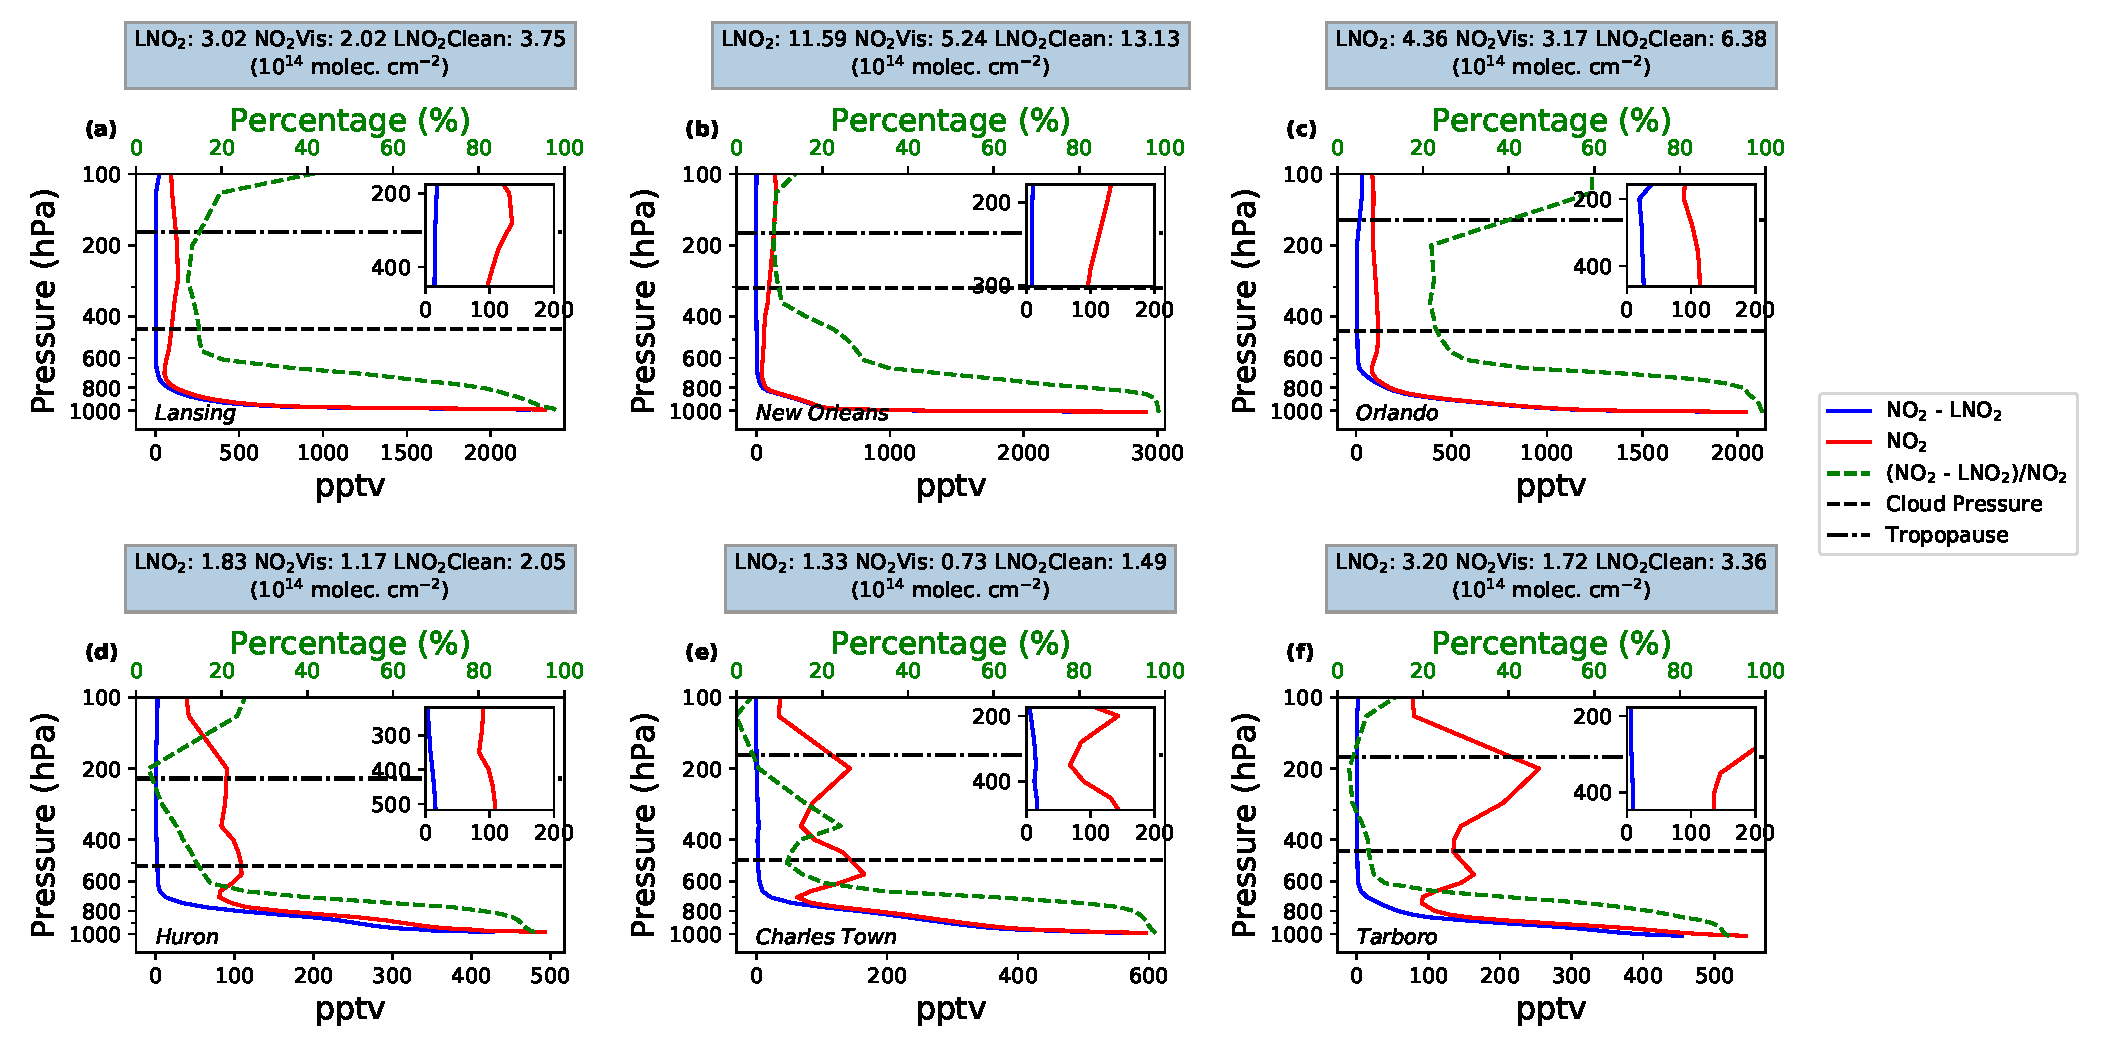
\includegraphics[width=18cm]{./figures/bkgd_comp.pdf}
\caption{在CRF $\geq$ 100\%条件下,六个网格中WRF-Chem 平均NO$_\textrm{2}$ 和背景 NO$_\textrm{2}$ 廓线。
顶行数据选自污染区域(图 \ref{fig:delta}(a)中的星号),而底行数据来自清洁区域(图 \ref{fig:delta}(a)中的三角形)。
绿色虚线是背景 NO$_\textrm{2}$ 与总 NO$_\textrm{2}$ 的平均比例廓线。
放大图显示了从云压到对流层顶的廓线。
标题基于\ref{section:amf_definition}节定义的三种不同方法估算得到的产量。\\
Figure \ref{fig:bkgd_comp}. Comparisons of mean WRF-Chem NO$_\textrm{2}$ and background NO$_\textrm{2}$ profiles in six grids with CRF $\geq$ 100\% on specific days during MJJA 2014.
The top row data are selected from polluted regions (stars in Fig. \ref{fig:delta}a) while the bottom row data are from clean regions (triangles in Fig. \ref{fig:delta}a).
The green dashed lines are the mean ratio profiles of background NO$_\textrm{2}$ to total NO$_\textrm{2}$.
The zoomed figures show the profiles from the cloud pressure to the tropopause.
The titles present the mean productions based on three different methods mentioned in Sect. \ref{section:amf_definition}.}
\label{fig:bkgd_comp}
\end{figure}


表\ref{table:production_comp}显示了6个城市三种方法之间的相对变化。
AMFLNO$_2$ (式\ref{AMFLNO2_crf100}) 和 AMFLNO$_2$Clean (式\ref{AMFLNO2Clean_crf100})之间的区别是分子:
$\int_{p_{\textrm cloud}}^{p_{\textrm tp}} w_{\textrm cloudy}(p) NO_2(p) \: dp$
和$\int_{p_{\textrm cloud}}^{p_{\textrm tp}} w_{\textrm cloudy}(p) LNO_2(p) \: dp$。
当 LNO$_2$ 的比例较高或区域较清洁时,相对差异较小(例如 5.0\%--12.0\%,图\ref{fig:bkgd_comp}(d)--(f))。
最大的相对差异(46.3\%)发生在上对流层中背景 NO$_2$ 所占比例一直较高的情况下(图\ref{fig:bkgd_comp}(c))。
因此,我们的方法对背景 NO$_2$ 不太敏感,更适用于受污染地区的对流情况。
相比之下,由于云层下方的 LNO$_2$,我们方法估算的产量大于基于 NO$_2$Vis 的产量。
当云层较高时,特别是 LNO廓线的峰值低于云层时(图\ref{fig:bkgd_comp}(b)),
相对差异较大(121.2\%),因为更多的 LNO$_2$ 不能包含在 NO$_2$Vis 中。
AMFLNO$_2$Clean (式\ref{AMFLNO2Clean_crf100}) 和 AMFNO$_2$Vis (式\ref{AMFNO2Vis_crf100}) 之间的相对变化取决于
$\int_{p_{\textrm cloud}}^{p_{\textrm tp}} w_{\textrm cloudy}(p) LNO_2(p) \: dp / \int_{p_{\textrm surf}}^{p_{\textrm tp}} w_{\textrm cloudy}(p) LNO_2(p) \: dp$,这也是受云影响,而不是背景NO$_2$。
其中最大的相对变化(153.8\%)发生在新奥尔良,它的云压最低,因此可见的柱密度最小。

图\ref{fig:cp_ratio_lno2}(a)为2014年5--8月在CRF$\geq$90\%的条件下,云压(CP)和LNO$_2$Vis与LNO$_2$比例的日分布。
当CP从600降低到300 hPa时,LNO$_2$Vis 与 LNO$_2$之比从 0.8 降低到 0.2,故在相对清洁的区域,NO$_2$Vis PE 小于 LNO$_2$ PE。
除了 LNO$_2$Vis,LNO$_2$ PE 也是受CP影响。
对于大于 30 mol每闪击的LNO$_2$ PE,CP 均小于 550 hPa(图\ref{fig:cp_ratio_lno2}(b)),
而较小的 LNO$_2$ PE(<30 mol每闪击)出现在 650 和 200 hPa 之间。
由于较高的LNO$_2$ PE 和闪电数据数量有限,现阶段我们无法推出 LNO$_2$ PE 与CP或其他闪电属性之间的关系。
由于CP仅代表云的发展,因此不能仅从CP值推导出闪电的垂直结构。
前人研究表示,闪电通道的长度会有所不同,并且取决于环境条件\citep{Carey.2016,Mecikalski.2017,Fuchs.2018}。
\citet{Davis.2019}比较了两种闪电:正常闪电和异常闪电。
一般来说,正常闪电是上层带正电和中层带负电,而异常闪电则相反\citep{Williams.1989}。
由于异常闪电中上升气流更强且闪电频率更高,因此异常闪电中的上对流层LNO$_x$浓度高于正常闪电。


\begin{table*}[h]
\scriptsize
\caption{基于相同先验廓线但不同估算方法时,产量的百分比变化\\Table \ref{table:production_comp}. The percent changes in the estimated production when using different methods based on the same a priori profiles.}
\begin{tabular}{clccc}
\hline
\textbf{} & \textbf{城市$^1$} & \textbf{(LNO$_\textrm{2}$Clean - LNO$_\textrm{2}$)/LNO$_\textrm{2}$} & \textbf{(LNO$_\textrm{2}$ - TropVis)/TropVis} & \textbf{(LNO$_\textrm{2}$Clean-TropVis)/TropVis} \\
\hline
\multirow{3}{*}{\textbf{污染地区}} & Lansing          & 24.2\%  & 49.5\%   & 85.6\%   \\
                                   & New Orleans      & 13.3\%  & 121.2\%  & 153.8\%  \\
                                   & Orlando          & 46.3\%  & 37.5\%   & 101.3\%  \\
\hline
\multirow{3}{*}{\textbf{清洁地区}}    & Huron            & 12.0\%  & 56.4\%   & 75.2\%   \\
                                   & Charles Town     & 12.0\%  & 82.2\%   & 104.1\%  \\
                                   & Tarboro          & 5.0\%   & 86.0\%   & 95.3\%   \\
\hline
\multicolumn{5}{l}{$^1$城市地址见图\ref{fig:delta}(a)。}\\
\multicolumn{5}{l}{$^1$Locations are denoted in Fig. \ref{fig:delta}(a).}
\end{tabular}
\label{table:production_comp}
\end{table*}

\subsection{不确定性分析} \label{susbec:china_uncertainty}

由于由LNO$_x$垂直分布引起的不确定性无法直接估算。
而模式中LNO$_x$的分布主要有两种方法:已通过对流输送重新分布的LNO$_x$廓线(对流后)和在对流输送重新分布之前LNO$_x$的廓线(对流前)\citep{Allen.2012,Luo.2017}。
然而,鉴于与其他 LNO$_x$ 研究相比结果的相似性,我们相信本文研究中基于对流后LNO$_x$廓线的1$^{\circ}$ $\times$ 1$^{\circ}$结果足以估计LNO$_x$的平均产量。

\begin{figure}[t]
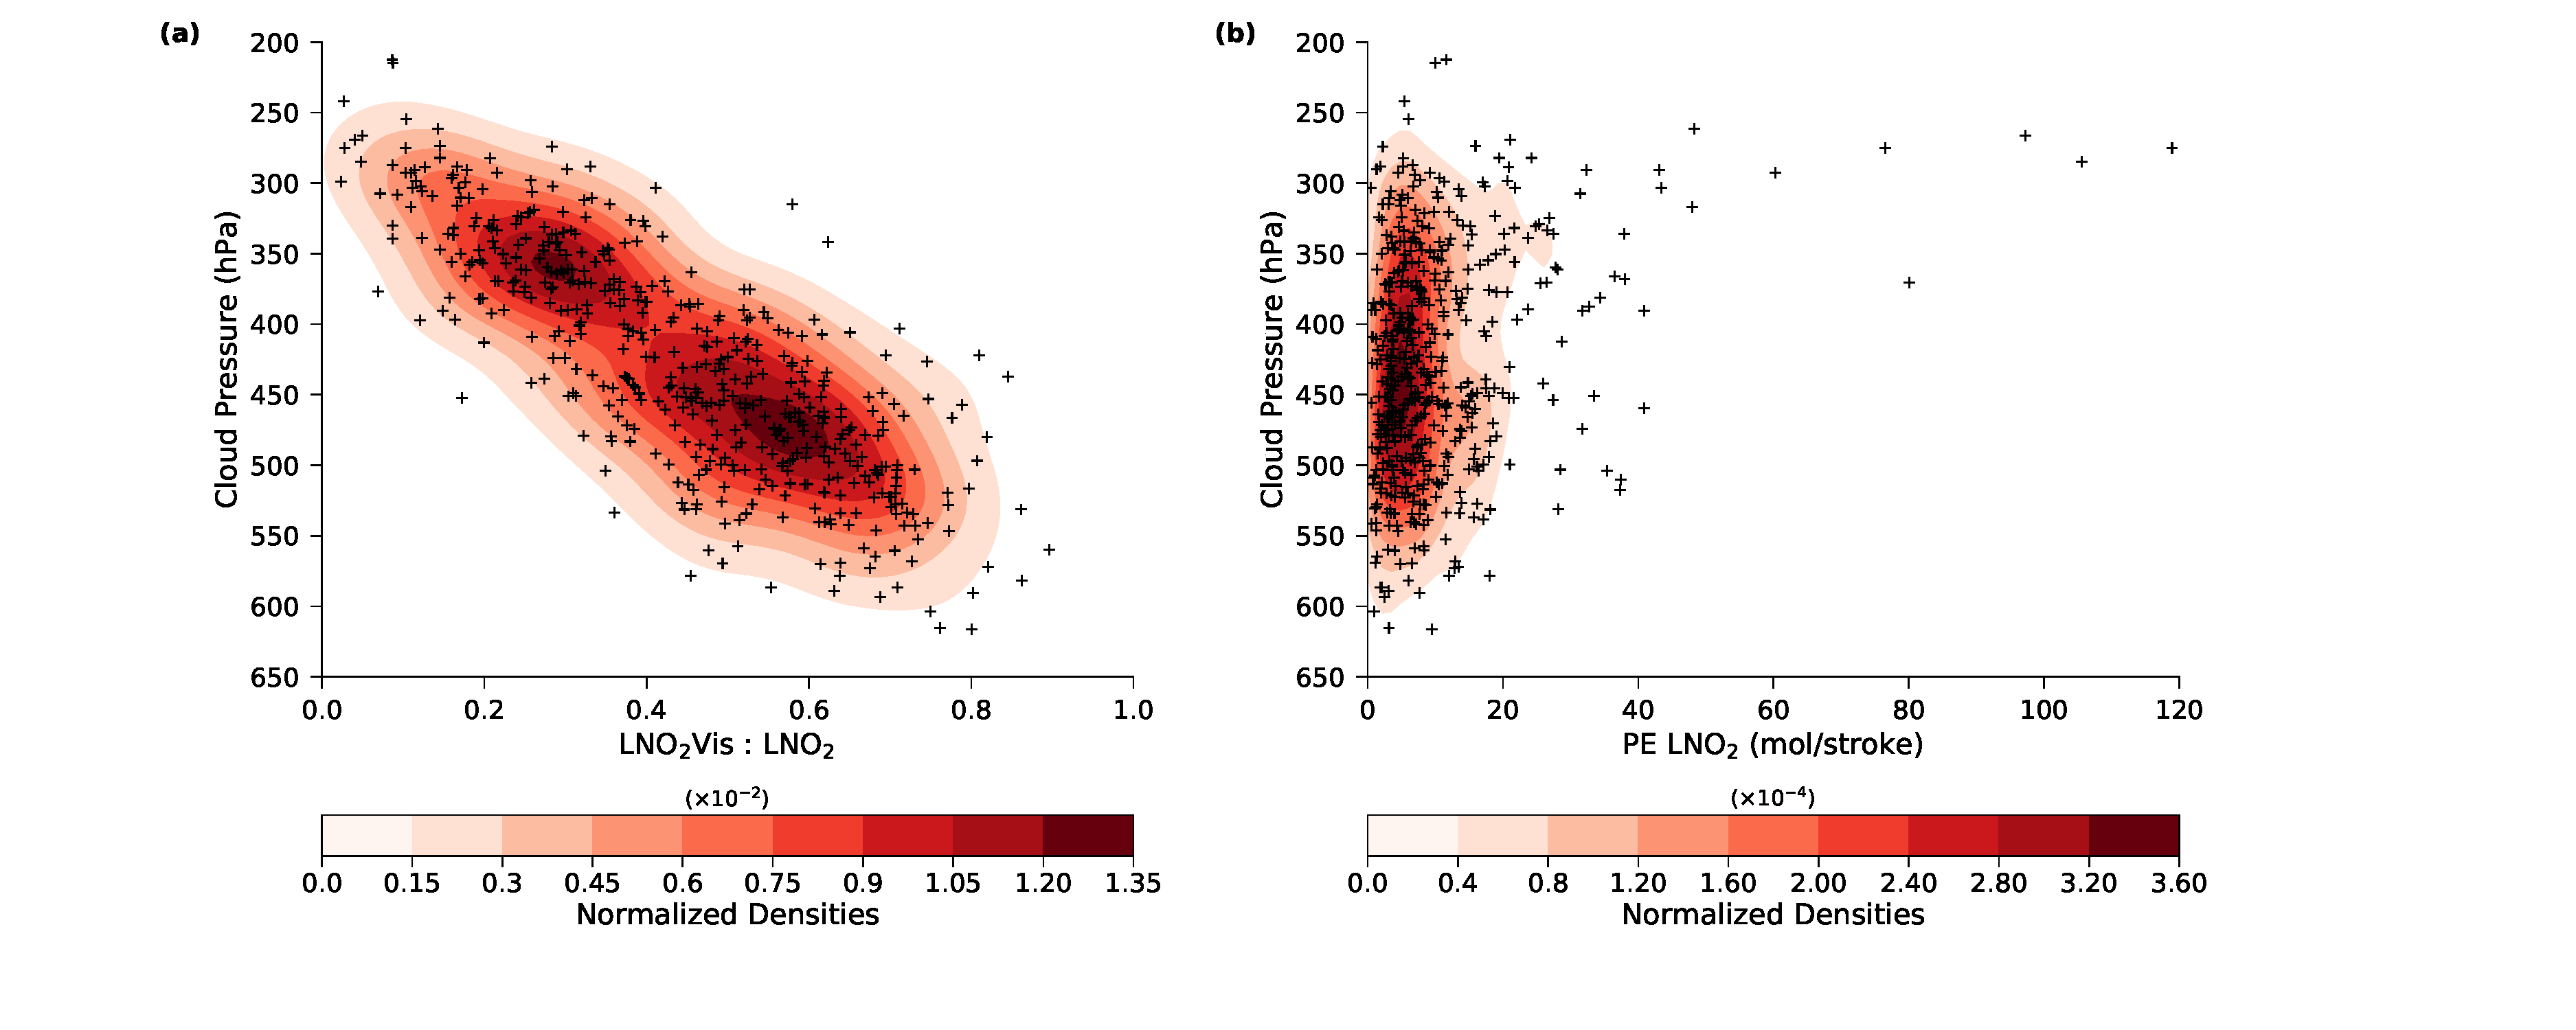
\includegraphics[width=15cm]{./figures/cp_ratio_lno2.pdf}
\caption{(a) LNO$_\textrm{2}$Vis 与 LNO$_\textrm{2}$之比的核密度估计(b)LNO$_\textrm{2}$产率与OMI测得的云压的核密度估计(2014年5--8月,CRF $\geq$ 90\%)。
内核密度估计是由名为 seaborn 的 Python 包中的 kdeplot 生成的。\\
Figure \ref{fig:cp_ratio_lno2}. Kernel density estimation of the (a) daily ratio of LNO$_\textrm{2}$Vis to LNO$_\textrm{2}$ and (b) daily LNO$_\textrm{2}$ production efficiency versus the daily cloud pressure measured by OMI with CRF $\geq$ 90\% for MJJA 2014.}
\label{fig:cp_ratio_lno2}
\end{figure}


\section{本章小结}
